\documentclass[tikz,margin=1mm]{standalone}


\begin{document}
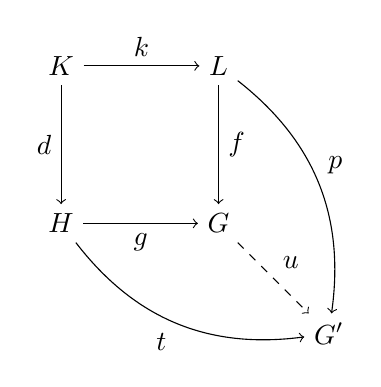
\begin{tikzpicture}[node distance=2cm, auto]
  \node (K) {$K$};
  \node[right of=K] (L) {$L$};
  \node[below of=K] (H) {$H$};
  \node[below of=L] (G) {$G$};
  \node[node distance=1.4cm, right of=G, below of=G] (G') {$G'$};

  \draw[->] (K) to node{$k$} (L);
  \draw[->] (K) to node[swap]{$d$} (H);
  \draw[->] (L) to node{$f$} (G);
  \draw[->] (H) to node[swap]{$g$} (G);

  \draw[->, bend left ] (L) to node{$p$} (G');
  \draw[->, bend right] (H) to node[swap]{$t$} (G');

  \draw[->, dashed] (G) to node{$u$} (G');

\end{tikzpicture}
\end{document}